% =====================================================================
%  Chapter 5 -- Taylor's Theories of Critical Distances
%
%  Baseline: d_b = 12 mm, L = 150 mm, f'c = 32 MPa, F_ref = 50 kN,
%            l_char = 20 mm, f_t = f_v = 0.5*sqrt(f'c) = 2.828 MPa.
%  Capacities and errors: from tcd_sensitivity / tcd_cost.csv, verified
%  against an independent reimplementation of the model.
%  Timings in Table 5.6: measured MATLAB values -- name the machine and
%  the MATLAB release in the caption.          % >>> STATE MACHINE <<<
% =====================================================================

\chapter{Taylor's Theories of Critical Distances}
\label{ch:tcd}

The Mode~II criterion of \eqref{eq:modeII} compares a hoop stress and a shear
stress against the tensile and shear strengths of the concrete. Applied
pointwise to the elastic field of Chapter~\ref{ch:method}, it predicts
cracking as soon as the peak of that field touches the strength. That peak is
both severe and highly localised: the stress concentration at the loaded end
decays over a short fraction of the bonded length, so a pointwise criterion
is governed by a state of stress that exists almost nowhere in the specimen.
The predicted capacity is accordingly far below anything measured, and it
falls further as the field is resolved more finely, because nothing in the
criterion fixes the scale over which the stress is to be judged. That
behaviour is the signature of a failure criterion with no length scale in
it.

The Theory of Critical Distances (TCD) supplies that length scale. Developed
by \textcite{taylorTheoryCriticalDistances2010}
from the earlier non-local proposals of Neuber and Peterson, it asserts that
failure is controlled not by the peak elastic stress but by the elastic
stress sampled over a finite region of material, whose size is the critical
distance $l_{\mathrm{ch}}$: a property of the material rather than of the
geometry.

The theory admits three standard forms, distinguished only by the geometry
over which the elastic field is sampled: the Point Method, the Line Method
and the Area Method. All three were implemented in the code and compared
against one another. This chapter sets out the theory and the implementation
of each in turn, and then examines how far each one's prediction depends on
the discretisation it requires rather than on the mechanics it represents.

The worked examples that follow all use the same specimen, evaluated in the
pull-push arrangement: a \SI{12}{\milli\metre} bar at \SI{150}{\milli\metre}
embedment in a \SI{150}{\milli\metre} concrete cylinder of
$f'_c = \SI{32}{\mega\pascal}$, so that
$f_t = f_v = 0.5\sqrt{f'_c} = \SI{2.828}{\mega\pascal}$ and
$F_{\mathrm{I}} = f_{sy}A_s = \SI{72.38}{\kilo\newton}$, with a critical
distance of $l_{\mathrm{ch}} = \SI{20}{\milli\metre}$ and every stress
evaluated at a reference load of $F_{\mathrm{ref}} = \SI{50}{\kilo\newton}$.
The full parameter set is listed in Table~\ref{tab:refspec}, where the same
specimen is carried into the sensitivity study.

% =====================================================================
\section{Three methods of Critical Distances}
\label{sec:threemethods}

\subsection{Area Method}
\label{sec:areamethod}
 
\subsubsection*{Theory}
 
The Area Method replaces the stress at a point by its mean over a semicircle
of radius $R = 1.32\,l_{\mathrm{ch}}$ centred on that point, the flat edge of
the semicircle lying on the free surface. For the bond problem the semicircle
lies in the $(z, r)$ plane and sits on the bar surface, since no material
exists below $r = r_s$.
 
The average is formed by dividing that half-disc into small squares of side
$l_{\mathrm{item}}$ and representing each square by the stress at its centre.
A square counts towards the average at station $z_0$ if its centre lies
within $R$ of $(z_0, r_s)$. Writing $N$ for the number of squares that
qualify and $(z_k, r_k)$ for their centres,
\begin{equation}
\label{eq:amavg}
\bar{\sigma}_\theta(z_0) = \frac{1}{N} \sum_{k=1}^{N} \sigma_\theta(z_k, r_k),
\qquad
\bar{\tau}_{rz}(z_0) = \frac{1}{N} \sum_{k=1}^{N} \tau_{rz}(z_k, r_k).
\end{equation}
Both stresses are averaged over the same squares, so the pair entering
\eqref{eq:modeII} is co-located by construction. Taking the stress at the
centre of each square is the midpoint rule, so \eqref{eq:amavg} approaches
the true mean over the semicircle as $l_{\mathrm{item}}$ is reduced; how
quickly it does so is the subject of Section~\ref{sec:meshload}.
 
The count $N$ is not the same at every station. Away from the ends the
half-disc is complete, but as $z_0$ approaches the loaded end part of it
falls outside the bonded length. Those squares do not exist, so they are not
counted and the divisor is reduced accordingly: the half-disc is
progressively clipped, as shown in Figure~\ref{fig:amsquares}. This matters
because the governing station in this model almost always lies at the loaded
end, so the average that decides the predicted capacity is usually taken over
a clipped half-disc rather than a complete one.
 
\begin{figure}[H]
  \centering
  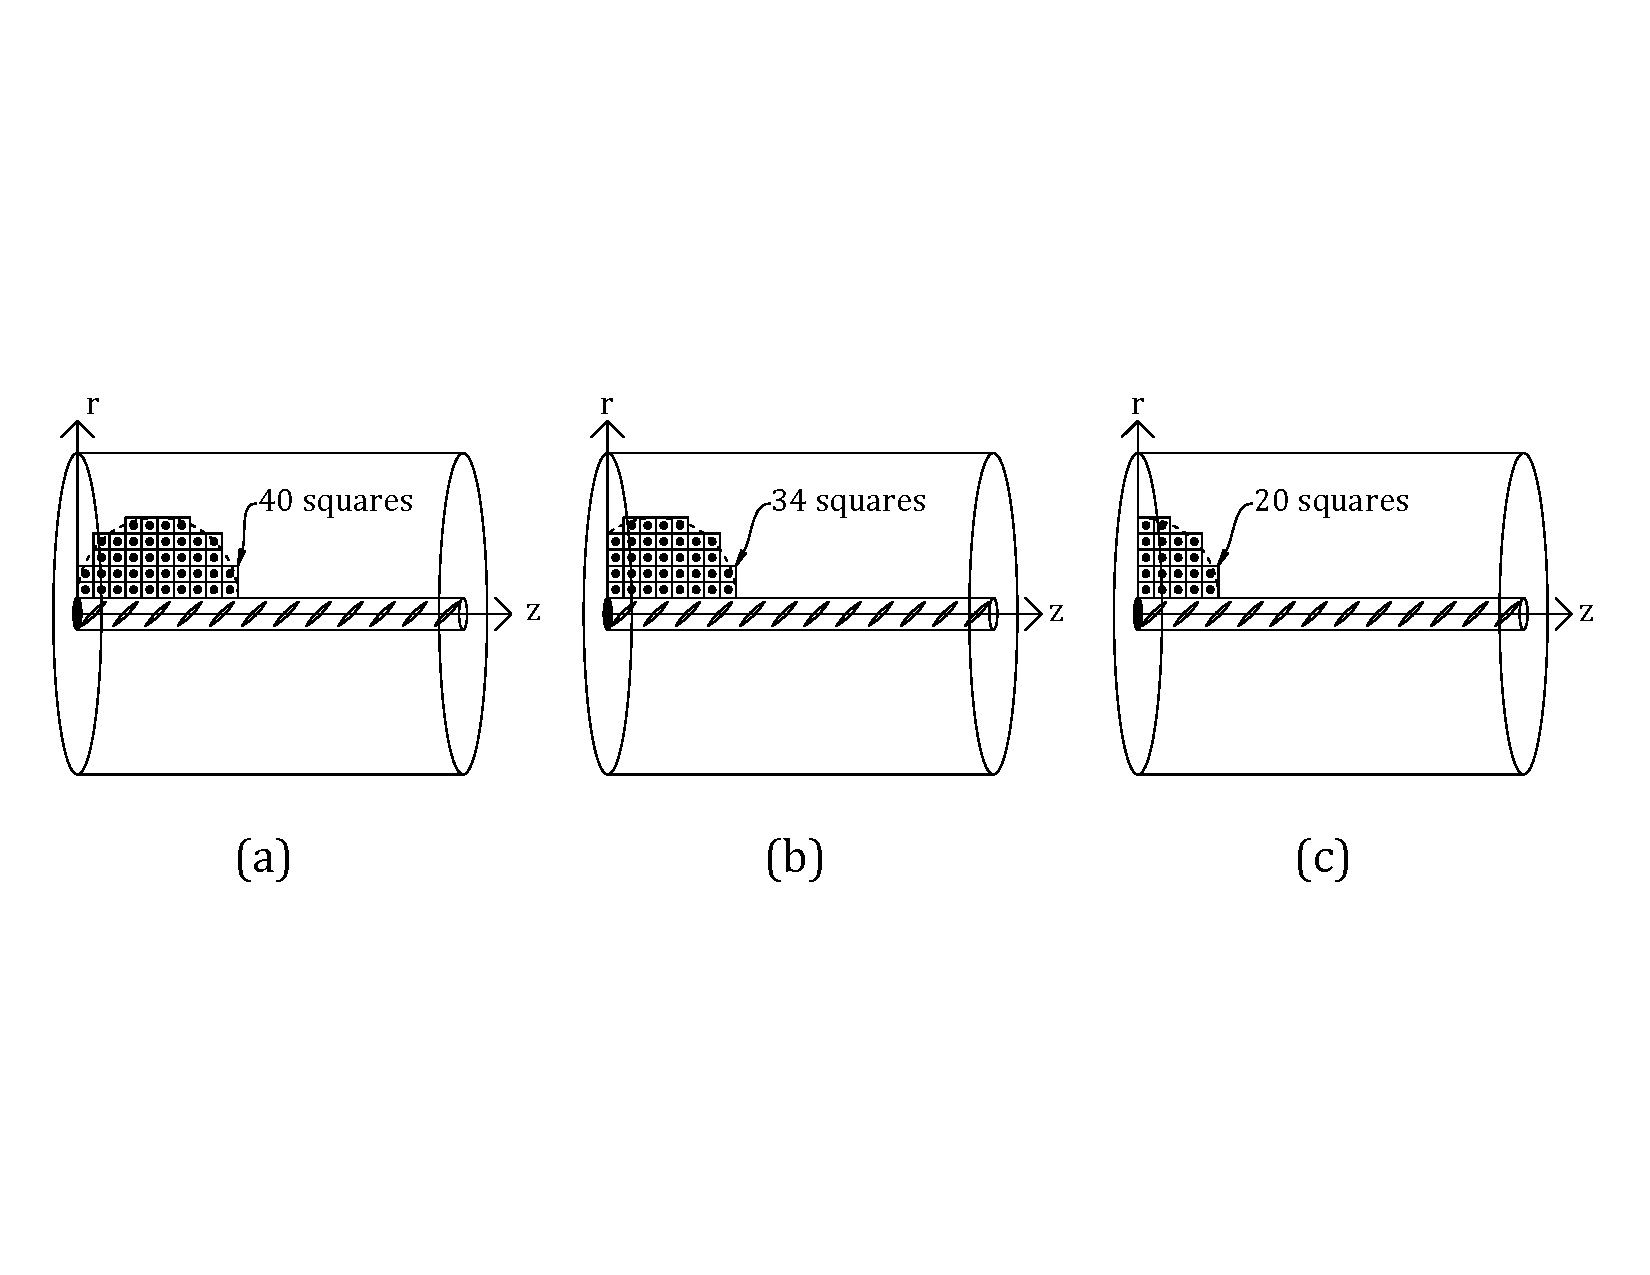
\includegraphics[width=\textwidth]{critical_distances_2}
  \caption[Clipping of the Area Method averaging region near the loaded
           end]{Area Method average at three stations along the bar. The
           half-disc of radius $R = 1.32\,l_{\mathrm{ch}}$ is tiled with
           squares of side $l_{\mathrm{item}}$, and a square counts only if
           its centre lies inside it. (a)~Complete region away from the ends;
           (b),~(c)~clipped as the station approaches the loaded end, where
           part of the region falls outside the bonded length. Counts are
           illustrative.}
  \label{fig:amsquares}
\end{figure}
 
Averaging in both the axial and the radial direction makes the Area Method
the only one of the three that responds to the axial gradient of the field,
which at the loaded end is far steeper than the radial gradient.
 
\subsubsection*{Implementation}
 
The solver follows the procedure set out in Chapter~\ref{ch:method} and
summarised there in Figure~\ref{fig:areamethod}: the averaging size is fixed,
the $(z, r)$ plane is tiled with squares, the set of squares admitted to the
half-disc is built once as a stencil, and that stencil is then placed at each
station in turn, clipped where it overruns the bonded length, averaged, and
converted to the Mode~II index, with only the governing station reported.
 
Two features of that implementation bear on what follows. Each square is
evaluated from the closed-form expressions of whichever layer its radius
falls in, the rib layer for $r \le r_r$ and the concrete beyond, so no
interpolation across the interface is involved and the average remains exact
in the sense that every sample is an exact value of the analytical field. And
the accuracy of \eqref{eq:amavg} is controlled by the single parameter
$l_{\mathrm{item}}$, which fixes both the resolution of the half-disc and the
spacing of the stations along the bar; it is the quantity refined in
Section~\ref{sec:meshload}.

\subsubsection*{Worked example}

With $l_{\mathrm{item}} = \SI{2}{\milli\metre}$ and
$R = 1.32 \times 20 = \SI{26.4}{\milli\metre}$, the tiling holds $75$
stations along the bar and $14$ radii outward from its surface, and a
complete half-disc contains $273$ squares. Sweeping \eqref{eq:amavg} along
the bar, the stresses at the maximum $\varphi_{\mathrm{II}}$ are

\begin{equation*}
\bar{\tau}_{rz} = \SI{8.818}{\mega\pascal},
\qquad
\bar{\sigma}_\theta = \SI{6.818}{\mega\pascal},
\end{equation*}

so that

\begin{equation*}
\varphi_{\mathrm{II},\max}
 = \left(\frac{6.818}{2.828}\right)^{2} + \left(\frac{8.818}{2.828}\right)^{2} - 1
 = 5.81 + 9.72 - 1 = 14.53,
\end{equation*}

and substituting into \eqref{eq:modeII},

\begin{equation*}
F_{\mathrm{II}} = \frac{F_{\mathrm{ref}}}{\sqrt{\varphi_{\mathrm{II},\max} + 1}}
 = \frac{50}{\sqrt{14.53 + 1}} = \SI{12.69}{\kilo\newton}.
\end{equation*}

Since $F_{\mathrm{II}} < F_{\mathrm{I}} = \SI{72.38}{\kilo\newton}$, Mode~II
governs and the predicted capacity is \SI{12.69}{\kilo\newton}, a mean bond
stress of $F_u/(\pi d_b L) = \SI{2.24}{\mega\pascal}$. Both squared terms are
substantial, the shear contributing $63\%$ and the hoop $37\%$: the governing
state is genuinely biaxial, and a criterion written on either component alone
would be unconservative by a quarter or more.

% ---------------------------------------------------------------------
\subsection{Line Method}
\label{sec:linemethod}
 
\subsubsection*{Theory}
 
The Line Method replaces the stress at a point by its mean along a straight
line of length $2\,l_{\mathrm{ch}}$ drawn from that point into the material.
Here the line is drawn radially outward from the bar surface, so that at
station $z$
\begin{equation}
\label{eq:lmcont}
\bar{\sigma}_\theta(z) = \frac{1}{2\,l_{\mathrm{ch}}}
  \int_{r_s}^{r_s + 2 l_{\mathrm{ch}}} \sigma_\theta(z, r)\ \mathrm{d}r,
\end{equation}
and identically for $\bar{\tau}_{rz}$. The method carries no axial averaging
at all: the value reported at $z$ depends only on the field in the plane $z$.
 
\subsubsection*{Implementation}
 
The method is the same device as the Area Method, reduced from a half-disc of
squares to a single row of steps along one radius, and is carried out as
follows.
 
\begin{enumerate}
\item \textbf{Set the averaging length.} The line runs radially outward from
      the bar surface over a distance $2\,l_{\mathrm{ch}}$, from $r_s$ to
      $r_s + 2\,l_{\mathrm{ch}}$. The solver checks that it stays inside the
      specimen, $r_s + 2\,l_{\mathrm{ch}} \le r_e$, which for a
      \SI{150}{\milli\metre} cylinder limits $l_{\mathrm{ch}}$ to
      \SI{34.5}{\milli\metre}.
 
\item \textbf{Divide the line into steps.} It is cut into
      $n_{\mathrm{item}}$ equal steps of width
      $\Delta r = 2\,l_{\mathrm{ch}}/n_{\mathrm{item}}$.
 
\item \textbf{Place a sample at the centre of each step,} at
      $r_i = r_s + \left(i - \tfrac{1}{2}\right)\Delta r$ for
      $i = 1 \dots n_{\mathrm{item}}$.
 
\item \textbf{Evaluate both stresses at every sampling radius,} taking
      $\tau_{rz}$ and $\sigma_\theta$ from the closed-form expressions of
      whichever layer the radius falls in: the rib layer for
      $r_i \le r_r$, the concrete beyond.
 
\item \textbf{Average the samples} to obtain the two values entering the
      index at that section,
      \begin{equation}
      \label{eq:lmgrid}
      \bar{\sigma}_\theta(z) \approx \frac{1}{n_{\mathrm{item}}}
        \sum_{i=1}^{n_{\mathrm{item}}} \sigma_\theta(z, r_i),
      \qquad
      \bar{\tau}_{rz}(z) \approx \frac{1}{n_{\mathrm{item}}}
        \sum_{i=1}^{n_{\mathrm{item}}} \tau_{rz}(z, r_i).
      \end{equation}
      Both are averaged over the same radii, so the pair is co-located by
      construction.
 
\item \textbf{Repeat at every station} on a uniform grid of $n_z = 801$
      points spanning $0 \le z \le L$. This axial grid is a separate
      discretisation from the sampling along the line and is held fixed
      throughout.
 
\item \textbf{Take the worst station.} The phi value is
      calculated at each $z$ and the largest value governs, giving the capacity
      from \eqref{eq:modeII}.
\end{enumerate}

\newpage
Sampling the step centres rather than the two ends of the line keeps every
sample strictly inside the averaging region. In particular the bar surface
itself is never sampled, which matters because the shear there is larger, and
the hoop stress less representative of the material around it, than anywhere
else on the line. It is also the more accurate choice: halving the step
divides the error by four, whereas a rule that includes both ends of the line
only halves it, because the two end points then carry more weight than they
should.
 
Five steps are enough. Because the hoop stress varies almost linearly along
the line, the rule converges quickly: raising $n_{\mathrm{item}}$ from $5$ to
$400$ moves the predicted capacity by only $0.1\%$. The quadrature along the
line is therefore not a meaningful source of error in this problem, and
$n_{\mathrm{item}} = 5$ is used throughout.
 
\subsubsection*{Worked example}
 
With $l_{\mathrm{ch}} = \SI{20}{\milli\metre}$ and $n_{\mathrm{item}} = 5$,
the line runs from $r_s = \SI{6}{\milli\metre}$ to \SI{46}{\milli\metre} in
steps of $\Delta r = \SI{8}{\milli\metre}$ and is sampled at the step
centres, $r = 10,\ 18,\ 26,\ 34,\ \SI{42}{\milli\metre}$. The index peaks at
the loaded end, $z_{\mathrm{cr}} = 0$, where the shear boundary condition
$\tau_{rz} = 0$ holds exactly and the hoop stress is at its maximum. The five
samples are listed in Table~\ref{tab:lmexample}.
 
\begin{table}[htbp]
\centering
\caption{Line Method sampling at the governing station $z = 0$, reference
         specimen of Table~\ref{tab:refspec}. The shear vanishes identically
         because $\tau_{rz} = 0$ is imposed at both ends of the bonded
         length.}
\label{tab:lmexample}
\begin{tabular}{rrr}
\toprule
$r$ (\si{\milli\metre}) & $\tau_{rz}$ (\si{\mega\pascal}) & $\sigma_\theta$ (\si{\mega\pascal}) \\
\midrule
10 & 0 & 24.224 \\
18 & 0 & 23.197 \\
26 & 0 & 21.614 \\
34 & 0 & 19.473 \\
42 & 0 & 16.775 \\
\midrule
\multicolumn{1}{r}{mean} & 0 & 21.057 \\
\bottomrule
\end{tabular}
\end{table}
 
Hence
\begin{equation*}
\varphi_{\mathrm{II},\max} = \left(\frac{21.057}{2.828}\right)^{2} + 0 - 1 = 54.42,
\qquad
F_{\mathrm{II}} = \frac{50}{\sqrt{54.42 + 1}} = \SI{6.72}{\kilo\newton}.
\end{equation*}

Figure~\ref{fig:lmsamples} shows the construction at that section: the two
stress components plotted against radius, the five sampled values marked on
them, and the resulting average drawn as a level.
 
\begin{figure}[H]
  \centering
  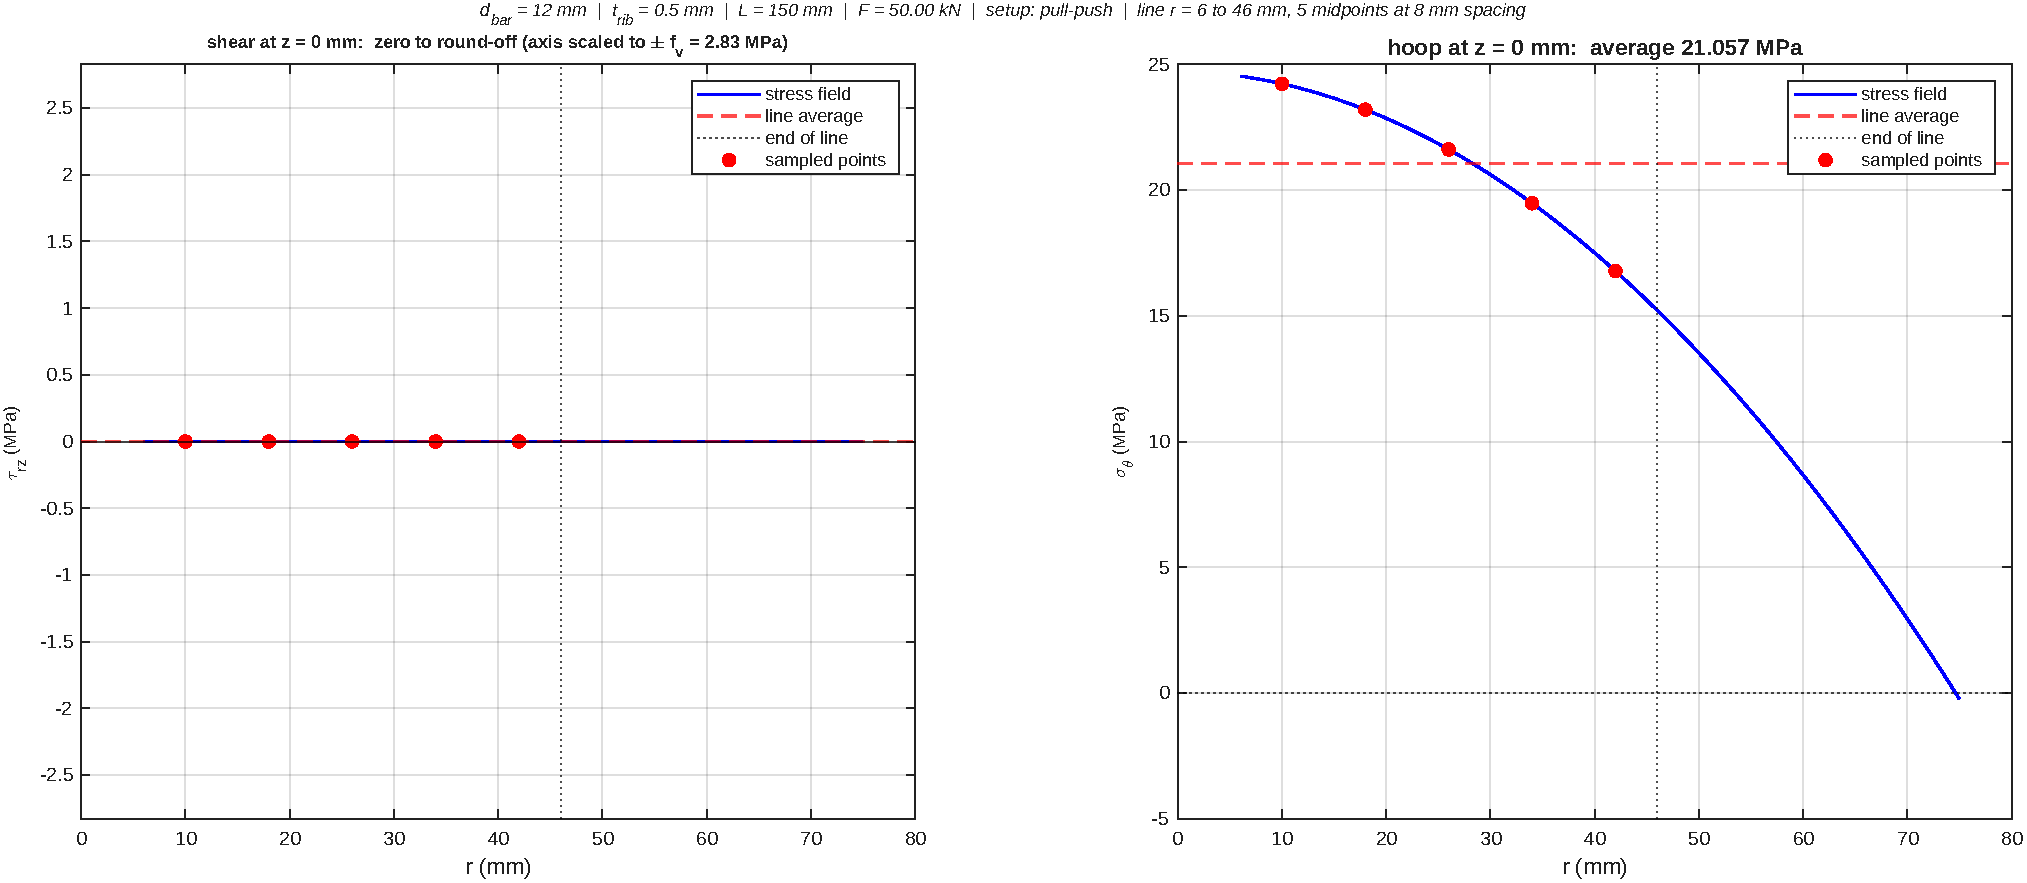
\includegraphics[width=\textwidth]{Line Method}
  \caption[Line Method sampling at the governing section]{The Line Method
           average at the governing section $z = 0$. Markers are the five
           step centres at $r = 10,\ 18,\ 26,\ 34,\ \SI{42}{\milli\metre}$,
           the dashed line their mean, and the dotted line the end of the
           averaging line at \SI{46}{\milli\metre}. Left: the shear, forced
           to zero at this section by the end boundary condition, plotted
           against $\pm f_v$. Right: the hoop stress, whose mean is
           \SI{21.06}{\mega\pascal}.}
  \label{fig:lmsamples}
\end{figure}

% ---------------------------------------------------------------------
\subsection{Point Method}
\label{sec:pointmethod}
 
\subsubsection*{Theory}
 
The Point Method performs no averaging at all. The stress entering
\eqref{eq:modeII} is the elastic stress evaluated at a single point a
distance $l_{\mathrm{ch}}/2$ from the stress raiser, measured here radially
outward from the bar surface:
\begin{equation}
\label{eq:pmcont}
\bar{\sigma}_\theta(z) = \sigma_\theta\!\left(z,\ r_{\mathrm{pt}}\right),
\qquad
\bar{\tau}_{rz}(z) = \tau_{rz}\!\left(z,\ r_{\mathrm{pt}}\right),
\qquad
r_{\mathrm{pt}} = r_s + \tfrac{1}{2} l_{\mathrm{ch}}.
\end{equation}
The offset preserves the non-local character of the criterion, so the
capacity still carries a length scale; what is lost is any smoothing, so the
prediction inherits whatever the sampling radius happens to pass through.
 
\subsubsection*{Implementation}
 
There is no quadrature, no stencil and no averaging window to choose: the two
closed-form expressions are evaluated once at $r = r_{\mathrm{pt}}$ and
substituted directly into \eqref{eq:modeII}. As in the Line Method the
layer expressions are selected by radius, and the solver halts if
$r_{\mathrm{pt}} > r_e$.
 
\subsubsection*{Worked example}
 
With $l_{\mathrm{ch}} = \SI{20}{\milli\metre}$ the sampling radius is
$r_{\mathrm{pt}} = \SI{16}{\milli\metre}$. The index again peaks at
$z_{\mathrm{cr}} = 0$, where the shear vanishes and
$\sigma_\theta = \SI{23.506}{\mega\pascal}$, giving
\begin{equation*}
\varphi_{\mathrm{II},\max} = \left(\frac{23.506}{2.828}\right)^{2} - 1 = 68.07,
\qquad
F_{\mathrm{II}} = \frac{50}{\sqrt{68.07 + 1}} = \SI{6.02}{\kilo\newton}.
\end{equation*}

% ---------------------------------------------------------------------
\subsection{Comparison of the three methods}
\label{sec:methodcompare}
 
Table~\ref{tab:threecompare} collects the three predictions.
 
\begin{table}[htbp]
\centering
\caption{The three critical-distance methods applied to the reference
         specimen of Table~\ref{tab:refspec}, $l_{\mathrm{ch}} =
         \SI{20}{\milli\metre}$. Stresses and $\varphi_{\max}$ are at the
         production discretisation; the last column is the converged value
         from Section~\ref{sec:sensitivity}.}
\label{tab:threecompare}
\begin{tabular}{lrrrrr}
\toprule
Method & $\bar{\tau}_{rz}$ & $\bar{\sigma}_\theta$ & $\varphi_{\max}$
       & $F_{\mathrm{II}}$ & converged \\
       & (\si{\mega\pascal}) & (\si{\mega\pascal}) & &
       (\si{\kilo\newton}) & (\si{\kilo\newton}) \\
\midrule
Point Method                                       &  0    & 23.51 & 68.07 &  6.02 &  6.02 \\
Line Method ($n_{\mathrm{item}} = 5$)              &  0    & 21.06 & 54.42 &  6.72 &  6.72 \\
Area Method ($l_{\mathrm{item}} = \SI{2}{\milli\metre}$) &  8.82 &  6.82 & 14.53 & 12.69 & 12.51 \\
\bottomrule
\end{tabular}
\end{table}
 
The Point and Line Methods agree closely with one another, while the Area
Method is roughly twice either of them: the spread between the three
converged predictions is $77\%$ of their mean. That is a very large
discrepancy for three methods calibrated to be identical, and the reason is
specific to the bond problem.
 
The three methods were calibrated on the field ahead of a sharp crack, which
decays the same way in every direction; sampling it along a line, over a
semicircle or at a single point therefore gives the same answer. The bond
field has no such symmetry. Along the bar the hoop stress collapses: at the
Point Method's sampling radius it falls from \SI{23.51}{\mega\pascal} at the
loaded end to \SI{2.14}{\mega\pascal} only \SI{15}{\milli\metre} in, and
reverses sign before \SI{20}{\milli\metre}. Across the radius it barely
changes, dropping $4\%$ over the first \SI{10}{\milli\metre}. The direction a
method averages in therefore decides its answer. The Area Method averages
along the bar as well as across it, so most of the hoop peak is averaged
away: its worst section moves off the loaded end, the shear term returns, and
the capacity doubles. The Point and Line Methods average only across the
radius, where there is almost nothing to average away.
 
This is why the Area Method is adopted for the remainder of this work. It is
the only one of the three that samples the axial gradient, and the axial
gradient is where the physics of the bond problem lies: the stress
concentration at the loaded end is a $z$-direction feature, not an
$r$-direction one. A further consequence is that the Point and Line Methods
are largely insensitive to the embedment length, since the state they sample
at $z = 0$ is governed by the end condition alone, whereas the Area Method's
average responds to how quickly the field decays into the bar.
 
The three methods also differ in how the governing mechanism is selected. For
the Area Method it depends on $l_{\mathrm{ch}}$: at \SI{5}{\milli\metre} the
half-disc is too small to reach the end hoop peak and the interior shear
maximum at $z = \SI{18.5}{\milli\metre}$ governs, whereas for
$l_{\mathrm{ch}} \ge \SI{10}{\milli\metre}$ the end region does. The Point
and Line Methods select $z = 0$ for every $l_{\mathrm{ch}}$ tested. The Area
Method is thus the only one in which the competition between the shear
mechanism along the bar and the splitting mechanism at the loaded end is
resolved by the model rather than fixed in advance.

% =====================================================================
\section{Sensitivity Analysis}
\label{sec:sensitivity}
 
Each of the three methods requires a discretisation, and each discretisation
introduces an error that has nothing to do with the mechanics. The Area
Method must tile its half-disc; the Line Method must place quadrature points
along its line; all three must sweep a grid of stations along the bar. This
section quantifies that error by refining each method's own discretisation
until its answer stops moving, and reporting how far every coarser run sits
from that converged value.
 
\subsection{Reference specimen}
\label{sec:refspec}
 
Every result in this chapter, both the worked examples of
Section~\ref{sec:threemethods} and the convergence study that follows, uses
the single configuration of Table~\ref{tab:refspec}, evaluated in the
pull-push arrangement. It is a \SI{12}{\milli\metre} bar embedded
\SI{150}{\milli\metre} into a \SI{150}{\milli\metre} concrete cylinder, so
the embedment is $12.5\,d_b$ and the cover is more than six bar diameters:
short enough that the stress distribution stays close to elastic up to
failure, and thick enough that the outer boundary does not control the hoop
stress at the bar surface.
 
\begin{table}[htbp]
\centering
\caption{Reference specimen used throughout this chapter.}
\label{tab:refspec}
\begin{tabular*}{\textwidth}{@{\extracolsep{\fill}}llr@{}}
\toprule
Quantity & Symbol & Value \\
\midrule
Bar diameter               & $d_b$              & \SI{12}{\milli\metre} \\
Rib layer thickness        & $t_{\mathrm{rib}}$ & \SI{0.5}{\milli\metre} \\
Concrete cylinder diameter & $d_{\mathrm{cyl}}$ & \SI{150}{\milli\metre} \\
Bonded length              & $L$                & \SI{150}{\milli\metre} \\
Bar modulus, Poisson ratio & $E_s,\ \nu_s$      & \SI{200}{\giga\pascal},\ 0.3 \\
Bar yield stress           & $f_{sy}$           & \SI{500}{\mega\pascal} \\
Concrete modulus, Poisson ratio & $E_c,\ \nu_c$ & \SI{30.1}{\giga\pascal},\ 0.2 \\
Concrete strength          & $f'_c$             & \SI{32}{\mega\pascal} \\
Tensile, shear strength    & $f_t = f_v = 0.5\sqrt{f'_c}$ & \SI{2.828}{\mega\pascal} \\
Reference load             & $F_{\mathrm{ref}}$ & \SI{50}{\kilo\newton} \\
Critical distance          & $l_{\mathrm{ch}}$  & \SI{20}{\milli\metre} \\
\midrule
Bar stress at $F_{\mathrm{ref}}$ & $f = F_{\mathrm{ref}}/A_s$ & \SI{442.1}{\mega\pascal} \\
Mode~I capacity            & $F_{\mathrm{I}} = f_{sy}A_s$ & \SI{56.55}{\kilo\newton} \\
\bottomrule
\end{tabular*}
\end{table}
 
Three conventions govern the study that follows. First, $l_{\mathrm{ch}}$ and
all specimen parameters are held at the values of Table~\ref{tab:refspec}, so
every difference reported here is numerical rather than physical. Second,
each method is measured against its \emph{own} finest run rather than against the
other methods: the gap between the three converged values quantified in
Section~\ref{sec:methodcompare} is a modelling choice, not a discretisation
error, and mixing the two would make both unreadable. Third, nothing is
re-derived between runs. The symbolic solution of
Chapter~\ref{ch:method} is obtained once and the four stress expressions
compiled to numerical functions once, so that refining a mesh changes only
how often those closed-form expressions are evaluated, never what they are.
 
\subsection{Mesh Size vs Pullout Load}
\label{sec:meshload}
 
\subsubsection*{Area Method}
 
Refinement means raising the number of steps $n_{\mathrm{item}}$ along the
line. The results are in Table~\ref{tab:sensline}.
 
\begin{table}[htbp]
\centering
\caption{Line Method: convergence of the predicted Mode~II capacity with the
         number of steps along the averaging line. Line length
         \SI{40}{\milli\metre}; each run averages the stress at the
         $n_{\mathrm{item}}$ step centres, as in \eqref{eq:lmgrid}.}
\label{tab:sensline}
\begin{tabular}{rrrr}
\toprule
$n_{\mathrm{item}}$ & step (\si{\milli\metre})
  & $F_{\mathrm{II}}$ (\si{\kilo\newton}) & error (\si{\percent}) \\
\midrule
  1 & 40.0 & 6.5432 & $-2.685$ \\
  2 & 20.0 & 6.6776 & $-0.685$ \\
  5 &  8.0 & 6.7163 & $-0.110$ \\
 10 &  4.0 & 6.7218 & $-0.027$ \\
 20 &  2.0 & 6.7232 & $-0.007$ \\
 50 &  0.8 & 6.7235 & $-0.002$ \\
100 &  0.4 & 6.7237 & ---      \\
\bottomrule
\end{tabular}
\end{table}
 
The rule converges from below and at second order: each halving of the step
divides the error by four. Convergence is from below because the samples never reach the bar
surface, where the hoop stress is highest, so every finite step
underestimates the mean slightly. In absolute terms the error is negligible
almost immediately: two steps are already within $0.7\%$ of the converged
\SI{6.7237}{\kilo\newton} and the production setting of five is within
$0.11\%$. Beyond about twenty steps the remaining differences are smaller
than the rounding in the fourth decimal place. The quadrature along the line
is therefore not a meaningful source of error in this problem, because the
radial variation it integrates is close to linear.
 
\subsubsection*{Line Method}
 
Refinement means raising the number of steps $n_{\mathrm{item}}$ along the
line. The results are in Table~\ref{tab:sensline}.
 
\begin{table}[htbp]
\centering
\caption{Line Method: convergence of the predicted Mode~II capacity with the
         number of steps along the averaging line. Line length
         \SI{40}{\milli\metre}; each run averages the stress at the
         $n_{\mathrm{item}}$ step centres, as in \eqref{eq:lmgrid}.}
\label{tab:sensline}
\begin{tabular}{rrrr}
\toprule
$n_{\mathrm{item}}$ & step (\si{\milli\metre})
  & $F_{\mathrm{II}}$ (\si{\kilo\newton}) & error (\si{\percent}) \\
\midrule
  1 & 40.0 & 6.5432 & $-2.685$ \\
  2 & 20.0 & 6.6776 & $-0.685$ \\
  5 &  8.0 & 6.7163 & $-0.110$ \\
 10 &  4.0 & 6.7218 & $-0.027$ \\
 20 &  2.0 & 6.7232 & $-0.007$ \\
 50 &  0.8 & 6.7235 & $-0.002$ \\
100 &  0.4 & 6.7237 & ---      \\
\bottomrule
\end{tabular}
\end{table}
 
The rule converges from below and at second order: each halving of the step
divides the error by four. Convergence is from below because the samples never reach the bar
surface, where the hoop stress is highest, so every finite step
underestimates the mean slightly. In absolute terms the error is negligible
almost immediately: two steps are already within $0.7\%$ of the converged
\SI{6.7237}{\kilo\newton} and the production setting of five is within
$0.11\%$. Beyond about twenty steps the remaining differences are smaller
than the rounding in the fourth decimal place. The quadrature along the line
is therefore not a meaningful source of error in this problem, because the
radial variation it integrates is close to linear.
 
\subsubsection*{Point Method}
 
The Point Method averages nothing, so it carries no quadrature error at all.
Its only discretisation is the set of sections at which the index is formed
while searching for the governing one, and for this specimen that search is
exact at every spacing tested: refining it by a factor of sixty-four returns
$F_{\mathrm{II}} = \SI{6.01631}{\kilo\newton}$ every time.
 
The reason is that the $\varphi$ value peaks at the loaded end and every grid begins at
the loaded end, so the governing section is sampled however coarse the
spacing is. This is not particular to one critical distance. Across the range
$l_{\mathrm{ch}} = \SIrange{5}{30}{\milli\metre}$ the hoop stress at the
loaded end dominates the index and the interior shear maximum never governs,
so the governing section stays at $z = 0$ throughout. The Point Method is
therefore mesh independent for this problem, and the spacing along the bar
can be as coarse as convenience allows.
 
That independence follows from where the maximum lies rather than from
anything in the method, and it would be lost if the governing section were
interior, as it is for the Area Method at small critical distances. A grid
deliberately offset by half a spacing, so that the loaded end is not sampled,
confirms as much: the predicted capacity then falls from \SI{7.03}{\kilo\newton}
to \SI{6.03}{\kilo\newton} as the spacing is refined, halving its error at
each step, because with no averaging to flatten the peak the error depends
entirely on how close the nearest section falls to it. The configurations
examined in this work do not produce that situation, but it is the reason the
axial spacing of the other two methods is held fixed rather than treated as
free.
 
\subsubsection*{Summary}
 
Table~\ref{tab:sensconv} collects the converged values and the coarsest mesh
that reaches $1\%$ of each.
 
\begin{table}[htbp]
\centering
\caption{Converged Mode~II capacities and the coarsest discretisation within
         $1\%$ of each.}
\label{tab:sensconv}
\begin{tabular}{llrr}
\toprule
Method & refinement parameter & coarsest within $1\%$
       & converged $F_{\mathrm{II}}$ (\si{\kilo\newton}) \\
\midrule
Area  & $l_{\mathrm{item}}$    & \SI{1}{\milli\metre}   & 12.508 \\
Line  & $n_{\mathrm{item}}$    & $2$                    &  6.724 \\
Point & section spacing        & any spacing tested     &  6.016 \\
\bottomrule
\end{tabular}
\end{table}
 
At any reasonable mesh the discretisation error of each method is an order of
magnitude smaller than the $77\%$ spread between the methods themselves. The
choice of averaging geometry therefore dominates the choice of mesh by a wide
margin, and the calibration of Chapter~[X] is a calibration of that choice
together with $l_{\mathrm{ch}}$, not of the numerics.
 
\subsection{Mesh Size vs Computation Time}
\label{sec:meshtime}
 
Cost is measured as the time to produce one value of
$F_{\mathrm{II}}$ for a given method and mesh: building the sampling grid,
evaluating the two stress fields on it, averaging, forming the index and
taking the worst station. The one-off symbolic derivation and the compilation
of the stress expressions are excluded, because they are shared by all three
methods and would swamp the comparison. Each case is repeated until at least
a fixed interval of wall clock has elapsed and the total divided by the
repeat count, so that the measurement is not limited by timer resolution.
 
\begin{table}[htbp]
\centering
\caption{Computation time per evaluation of $F_{\mathrm{II}}$ against mesh
         refinement, with the discretisation error of
         Section~\ref{sec:meshload} alongside.
         Times measured on an Intel
         Core i9-12900H (20 logical cores, \SI{2.5}{\giga\hertz}, 32\,GB
         RAM) running MATLAB R2026b under Windows~11.}
\label{tab:senstime}
\begin{tabular}{llrrr}
\toprule
Method & Mesh & Items per station
       & error (\si{\percent}) & time (\si{\milli\second}) \\
\midrule
Area  & $l_{\mathrm{item}} = \SI{4}{\milli\metre}$    &    69 & $+3.85$ &   0.29 \\
Area  & $l_{\mathrm{item}} = \SI{2}{\milli\metre}$    &   273 & $+1.43$ &   0.55 \\
Area  & $l_{\mathrm{item}} = \SI{1}{\milli\metre}$    &  1092 & $+0.56$ &   2.67 \\
Area  & $l_{\mathrm{item}} = \SI{0.75}{\milli\metre}$ &  1947 & $+0.43$ &   5.70 \\
Area  & $l_{\mathrm{item}} = \SI{0.5}{\milli\metre}$  &  4383 & $+0.29$ &  21.93 \\
Area  & $l_{\mathrm{item}} = \SI{0.25}{\milli\metre}$ & 17516 & ---     & 139.79 \\
\midrule
Line  & $n_{\mathrm{item}} = 2$   &   2 & $-0.685$ & 0.23 \\
Line  & $n_{\mathrm{item}} = 10$  &  10 & $-0.027$ & 0.31 \\
Line  & $n_{\mathrm{item}} = 50$  &  50 & $-0.002$ & 0.39 \\
Line  & $n_{\mathrm{item}} = 100$ & 100 & ---      & 0.50 \\
\midrule
Point & For all values & 1 & --- & 0.041 \\
\bottomrule
\end{tabular}
\end{table}
 
Three features of Table~\ref{tab:senstime} matter for the way the model is
used.
 
The Area Method's cost grows as $l_{\mathrm{item}}^{-3}$. Halving the item
side multiplies the work eightfold, because the number of items inside the
half-disc grows as $l_{\mathrm{item}}^{-2}$ while the number of stations at
which that average must be formed grows as $l_{\mathrm{item}}^{-1}$. The
measured cost bears this out: refining from \SI{1}{\milli\metre} to
\SI{0.25}{\milli\metre} raises the time from \SI{2.67}{\milli\second} to
\SI{139.79}{\milli\second}, a factor of $52$ against the $64$ predicted, and
the times rise monotonically across the whole range. Combined with the
first-order convergence of Section~\ref{sec:meshload}, cubic cost growth
means the Area Method's cost rises as the inverse cube of the accuracy
demanded: cutting the discretisation error by ten costs a thousandfold in
time.
 
The Line and Point Methods are effectively free by comparison. The Line
Method's cost is almost flat below $n_{\mathrm{item}} = 50$ because it is
dominated by the fixed axial grid rather than by the sampling along the line,
and the Point Method's cost is simply that of evaluating two closed-form
expressions at every section. Both remain below \SI{0.6}{\milli\second} at
every mesh tested, more than two orders of magnitude below the Area Method's
finest run.
 
Most importantly, the accuracy actually required is cheap in every case. The
coarsest mesh within $1\%$ of the converged value costs
\SI{2.67}{\milli\second} for the Area Method against
\SI{139.79}{\milli\second} for the finest run, a saving of a factor of $52$;
for the Line Method the corresponding figures are \SI{0.23}{\milli\second}
against \SI{0.50}{\milli\second}. Running each method at its finest tested
mesh buys at most $0.6$ percentage points of accuracy for one to two orders
of magnitude in time.
 
This matters because the model is not run once. The calibration of
$l_{\mathrm{ch}}$ in Chapter~[X] evaluates the Mode~II capacity across a
database of specimens, and the parametric study of Chapter~[X] sweeps bar
diameter, embedment length and concrete strength, so a single capacity
evaluation is executed thousands of times. At
$l_{\mathrm{item}} = \SI{1}{\milli\metre}$ a sweep of \num{10000} cases costs
under half a minute, against roughly \SI{23}{\minute} at
\SI{0.25}{\milli\metre}, for a difference of less than one percent in every
predicted capacity. The working value $l_{\mathrm{item}} =
\SI{1}{\milli\metre}$ is adopted on that basis.
 
These times exclude the symbolic solution itself, which is obtained once per
specimen configuration and dominates the total runtime of the solver. On the
evidence of Table~\ref{tab:senstime} the discretisation of the
critical-distance averaging is not a bottleneck in this model at any mesh
accurate enough to use.